% Autor: Leonhard Segger, Alexander Neuwirth
% Datum: 2017-10-30
\documentclass[
	% Papierformat
	a4paper,
	% Schriftgröße (beliebige Größen mit „fontsize=Xpt“)
	12pt,
	% Schreibt die Papiergröße korrekt ins Ausgabedokument
	pagesize,
	% Sprache für z.B. Babel
	ngerman
]{scrartcl}

% Achtung: Die Reihenfolge der Pakete kann (leider) wichtig sein!
% Insbesondere sollten (so wie hier) babel, fontenc und inputenc (in dieser
% Reihenfolge) als Erstes und hyperref und cleveref (Reihenfolge auch hier
% beachten) als Letztes geladen werden!

%Malen
\usepackage{tikz}
\usetikzlibrary{calc,patterns,angles,quotes} % loads some tikz extensions\usepackage{tikz}
\usetikzlibrary{babel}

% Silbentrennung etc.; Sprache wird durch Option bei \documentclass festgelegt
\usepackage{babel}
% Verwendung der Zeichentabelle T1 (Sonderzeichen etc.)
\usepackage[T1]{fontenc}
% Legt die Zeichenkodierung der Eingabedatei fest, z.B. UTF-8
\usepackage[utf8]{inputenc}
% Schriftart
\usepackage{lmodern}
% Zusätzliche Sonderzeichen
\usepackage{textcomp}

% Mathepaket (intlimits: Grenzen über/unter Integralzeichen)
\usepackage[intlimits]{amsmath}
% Ermöglicht die Nutzung von \SI{Zahl}{Einheit} u.a.
\usepackage{siunitx}
% Zum flexiblen Einbinden von Grafiken (\includegraphics)
\usepackage{graphicx}
% Abbildungen im Fließtext
\usepackage{wrapfig}
% Abbildungen nebeneinander (subfigure, subtable)
\usepackage{subcaption}
% Funktionen für Anführungszeichen
\usepackage{csquotes}
\MakeOuterQuote{"}
% Zitieren, Bibliografie
\usepackage[sorting=none]{biblatex}


% Zur Darstellung von Webadressen
\usepackage{url}
%chemische Formeln
\usepackage[version=4]{mhchem}
% siunitx: Deutsche Ausgabe, Messfehler getrennt mit ± ausgeben
\usepackage{floatrow}
\floatsetup[table]{capposition=top}
\usepackage{float}
% Verlinkt Textstellen im PDF-Dokument
\usepackage[unicode]{hyperref}
% "Schlaue" Referenzen (nach hyperref laden!)
\usepackage{cleveref}
\sisetup{
	locale=DE,
	separate-uncertainty
}
\bibliography{BA-C-04_EDX_22-10-2018_References}


\begin{document}
	
	\begin{titlepage}
		\centering
		{\scshape\LARGE Versuchsbericht zu \par}
		\vspace{1cm}
		{\scshape\huge EDX - Energiedispersive Röntgenspektroskopie \par}
		\vspace{2.5cm}
		{\LARGE Gruppe BA-C-04 \par}
		\vspace{0.5cm}
		
		{\large Alexander Neuwirth (E-Mail: a\_neuw01@wwu.de) \par}
		{\large Leonhard Segger (E-Mail: l\_segg03@uni-muenster.de) \par}
		\vfill
		
		durchgeführt am 22.10.2018\par
		betreut von\par
		{\large Johann Preuß} %TODO Johann Adrian Preuß? Irrelephant?!? Neeeee!
		
		\vfill
		
		{\large \today\par}
	\end{titlepage}
	\tableofcontents
	\newpage

	%TODO mehr TODO in Default	

	\section{Kurzfassung}
	%TODO Hypothese	und deren Ergebnis, wenn Hypothese ist, dass nur Theorie erfüllt, sagen: Erwartung: Theorie aus einführung (mit reflink) erfüllt
	%TODO Ergebnisse, auch Zahlen, mindestens wenn's halbwegs Sinn ergibt
	%TODO Was wurde gemacht
	Die Energiedispersive Röntgenspektroskopie ist ein Verfahren, welches es den Materialwissenschaften erlaubt mithilfe des von einer Probe, die von einem Röntgenstrahl mit kontinuierlichem Spektrum beschossen wird, ausgesandten Röntgenfluoreszenzspektrums die Zusammensetzung der Probe zu bestimmen.
	Es sollen mithilfe eines Röntgengeräts und einigen bekannten Proben Röntgenfluoreszenzspektren verschiedener unbekannter Proben aufgezeichnet werden.%sollen kann man denke ich so benutzen...
	Auf Basis dieser Spektren wird die elementare Zusammensetzung der unbekannten Proben untersucht, wobei nicht nur die Art der vorkommenden Elemente, sondern auch ihr prozentualer Anteil an der Gesamtprobe bestimmt wird. %TODO ist das zweite Komma richtig?
	Zusätzlich kann das Moseleysche Gesetz bestätigt werden und die Abschirmkonstanten von sechs Elementen werden bestimmt. %TODO hoffentlich...
	
	%\section{Einführung} %optional
	
	
	\section{Methoden}
	Für die Versuchsdurchführung werden ein Röntgengerät, ein Vielkanalanalysator und verschiedene Proben größtenteils unbekannter Natur verwendet. %X-ray unit, 35 kV, basic unit
	Das Röntgengerät, welches mit einer Eisen-Anode arbeitet, und die Proben sind in \cref{fig_aufbau} dargestellt.
	Röntgenphotonen können durch eine Blende in die Versuchskammer eintreten, in der sich ein Probenhalter und eine PIN-Diode befinden.
	Die Diode ist mit dem Vielkanalanalysator verbunden.
	Hier wird ausgenutzt, dass die Anzahl der in der Detektordiode erzeugten Elektron-Loch-Paare als proportional zur Energie des eingetretenen Röntgenphotons angenommen werden kann. %TODO das ist doch richtig wiedergegeben, oder?
	Das Röntgengerät wird mit einer Spannung von \SI{35}{\kilo \electronvolt} betrieben, weshalb dies die maximal erwartbare messbare Energie ist.
	Zunächst wird der Probenhalter in einen Winkel von \SI{45}{\degree} und der Detektor in einen Winkel von \SI{90}{\degree} zum Röntgenstrahl gebracht.
	Diese Winkel werden mit dem Auge abgeschätzt, da die Verwendung des eingebauten Goniometers zu einer Stellung führt, die nach Augenmaß nicht dem gewünschten Winkel entspricht.
	
	Um dem verwendeten Messprogramm zu erlauben, den Proportionalitätsfaktor zwischen entstandenen Elektron-Loch-Paaren und Energie des Röntgenphotons zu bestimmen, wird mit zwei Proben, von denen bekannt ist, aus welchen Elementen sie bestehen, kalibriert.
	Zur Kalibrierung wird Eisen und Molybdän verwendet.
	Dann werden die Röntgenfluoreszenzspektren aller Proben aufgezeichnet und jeweils Gauß-Fits über die Peaks durchgeführt.
	Die Fitparameter werden verwendet, um Energie, Standardunsicherheit und Höhe des Peaks zu bestimmen.
	Nun können mithilfe dieser Werte und bekannten Übergangsenergien in verschiedenen Elementen die Zusammensetzungen der Proben untersucht bzw. überprüft werden.
	
	%TODO Eisen Kathode erwähnen?
	
	\begin{figure}[H]
		\centering
		\begin{subfigure}[t]{0.5\textwidth}
			\centering
			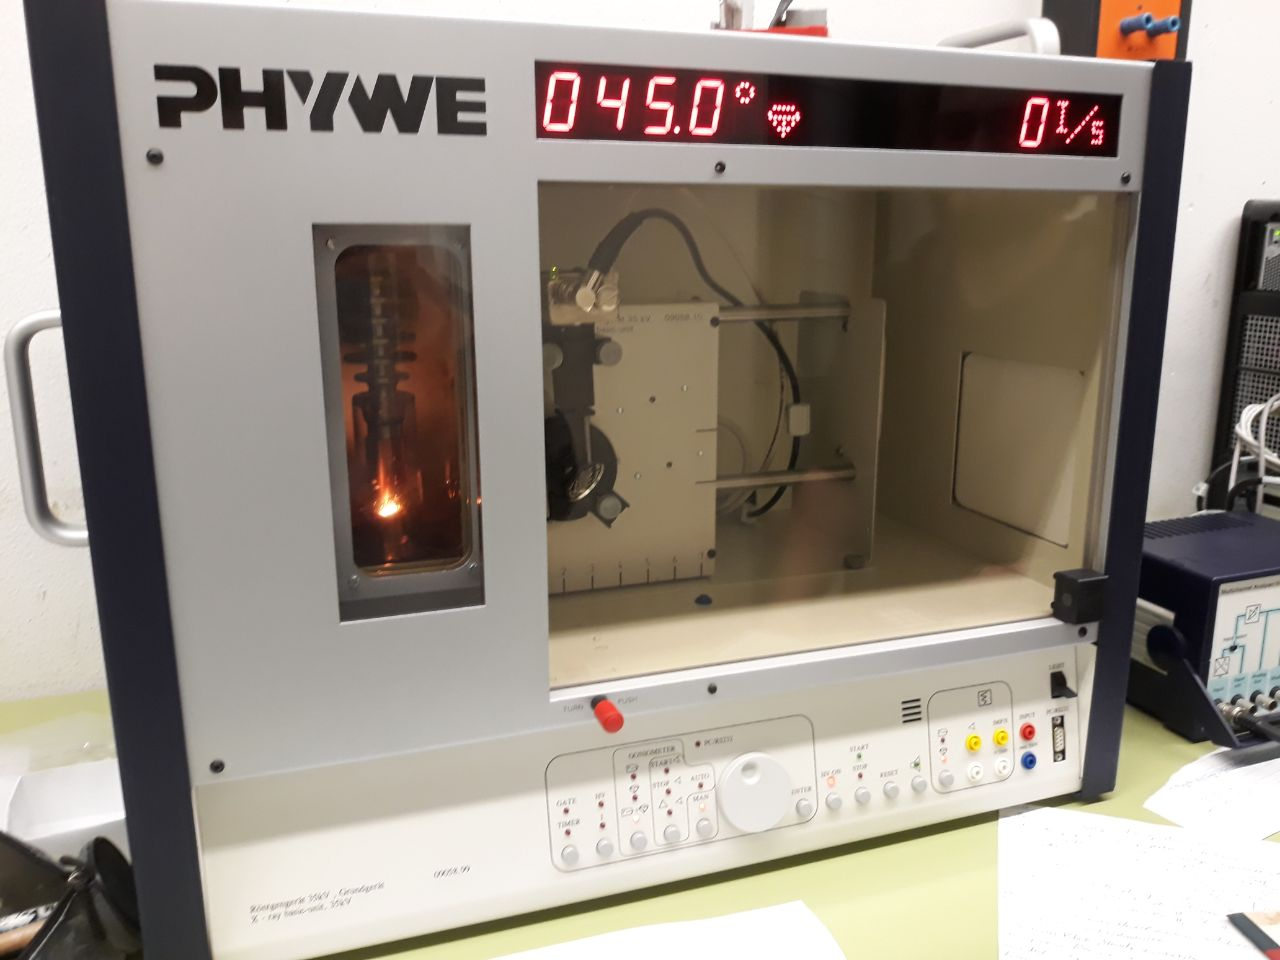
\includegraphics[width=1\textwidth]{images/aufbau}
			\label{fig_aufb_geraet}
			\caption{Röntgengerät}
		\end{subfigure}%
		\begin{subfigure}[t]{0.5\textwidth}
			\centering
			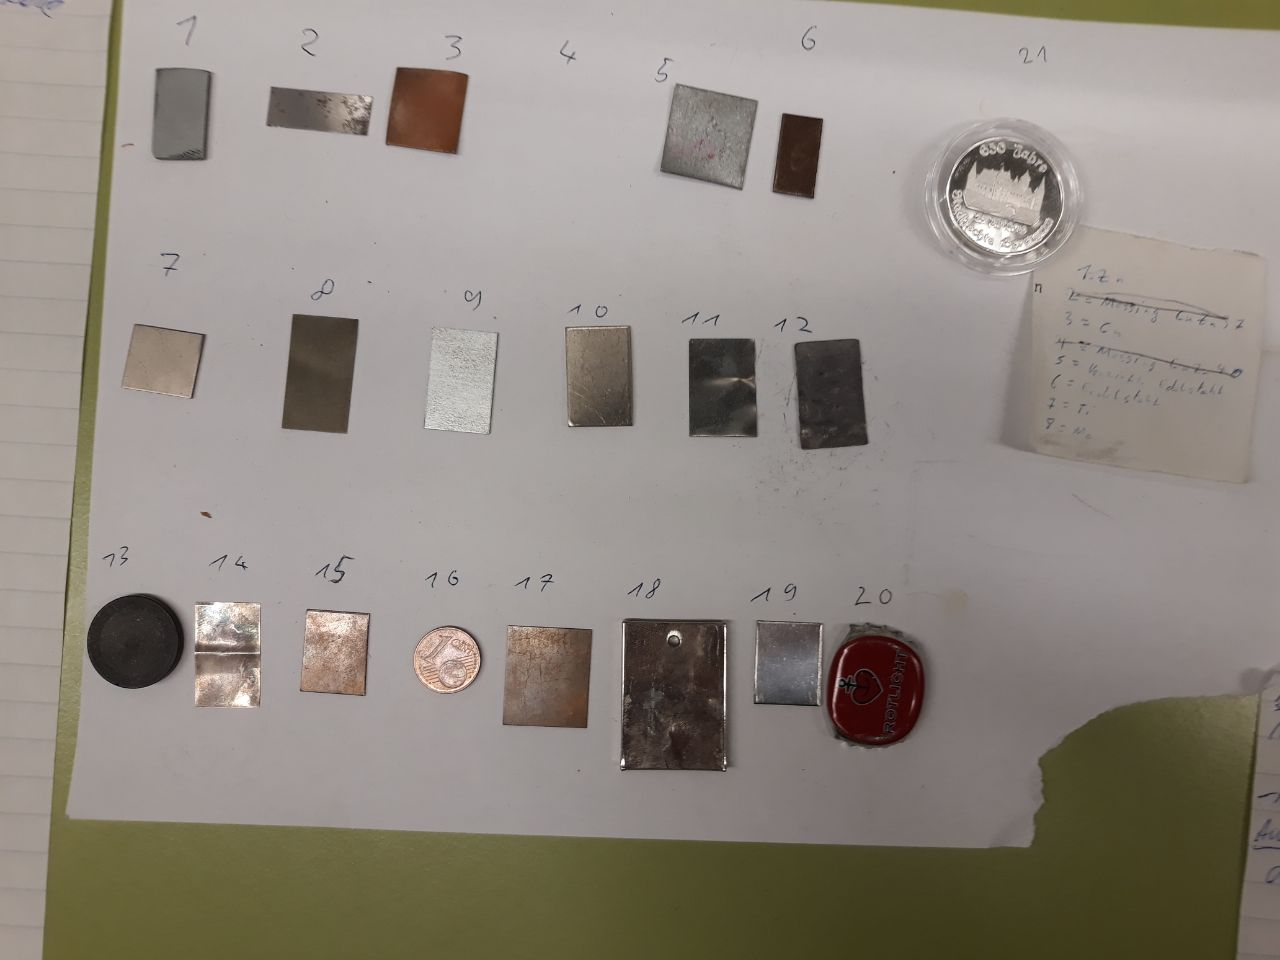
\includegraphics[width=1\textwidth]{images/proben}
			\label{fig_aufb_proben}
			\caption{Proben}
		\end{subfigure}
		\caption{
			\label{fig_aufbau}
			Verwendetes Röntgengerät und Proben. Die Probe mit der Nummer Vier ist nicht im Bild, da sie zum Zeitpunkt der Aufnahme gerade gemessen wurde.}%TODO Ist das wichtig zu erwähnen?
		\centering
		
	\end{figure}
	
	\section{Ergebnisse und Diskussion}
	%TODO Unsicherheiten
	

	\subsection{Beobachtung}
	%TODO Einflüsse von veränderten Parametern auf Messung
	
	\begin{figure}[H] %TODO von Logik: das hier woanders hin. 
		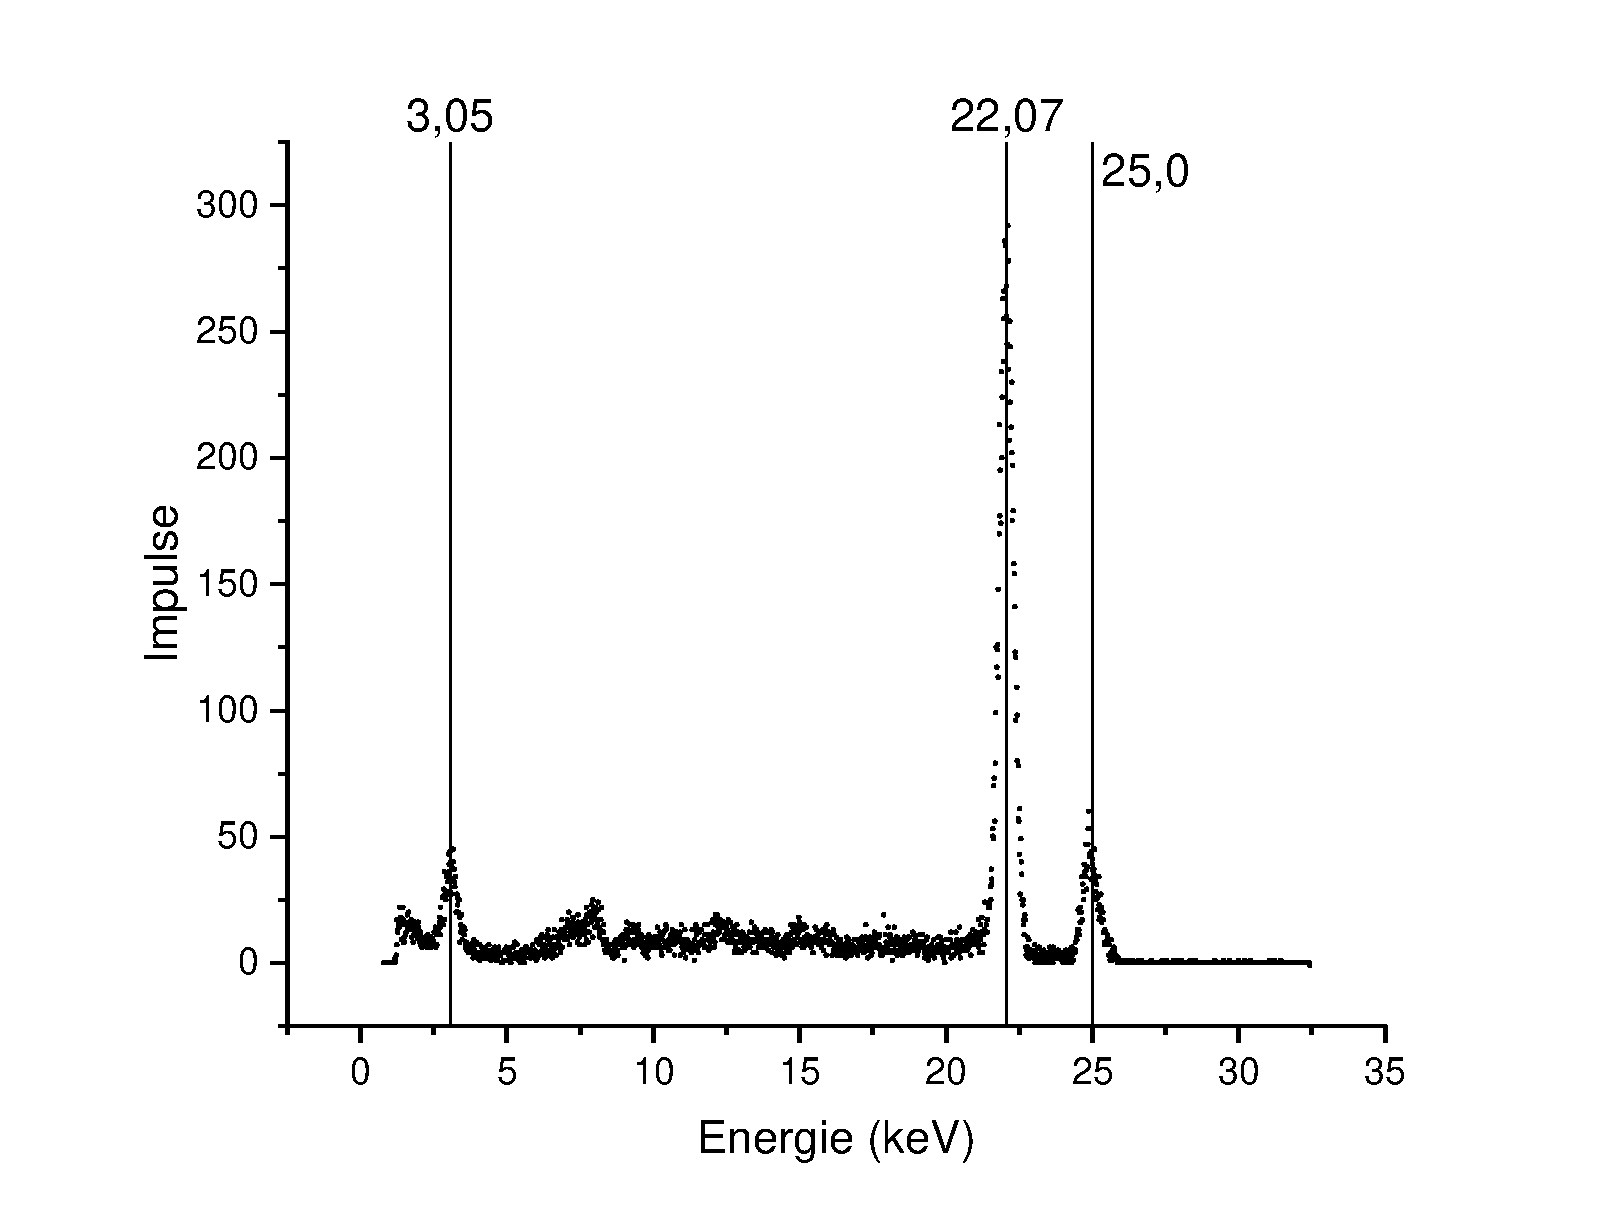
\includegraphics[width=0.9\textwidth]{images/Silbermuenze}
		\centering
		\caption{Röntgenfluoreszenzspektrum einer Silbermünze. Die Peaks der $\text{L}_\alpha$, $\text{K}_\alpha$ und $\text{K}_\beta$ Linien sind deutlich zu erkennen. Abseits dieser Peaks sind mehrere weitere signifikante Abweichungen von Null zu erkennen.} %TODO Das muss man vermutlich erklären, wenn man es erwähnt.
		\label{fig_ag_plot}
		\centering
	\end{figure} %TODO noch eins für Legierung
	
	\subsubsection{Unsicherheiten} %TODO GGF IN DATENANYLSY
	\subsection{Datenanalyse}
	\subsubsection{Bestimmung der Abschirmkonstanten}
	%TODO Berechung nach Aufgabenstellung
	Aus den gemessenen Energiespektren wurden die Energien der Peaks mittels eines Gauß-Fits bestimmt.
	Die Standardabweichung ergibt sich dabei aus der FWHM: %TODO ich denke, man sollte einmal schreiben wofür das steht.
	\begin{equation}
		\sigma = \frac{\text{FWHM}}{2\sqrt{\ln 2}}
	\end{equation}
	Die Ergebnisse sind in \cref{tb_peaks_known} und \cref{tb_peaks_unknown} aufgeführt.
	
	%TODO sortieren nach enrgie oder Ausprägung
	
	\begin{table}[H]
		\centering
		\resizebox{\textwidth}{!}{
		\begin{tabular}{ c | c || c | c | c }
			Probe (Angabe)&Energie $E_\text{Mess}$ in \SI{}{keV} & Element & char. Übergang &  Energie $E_\text{NIST}$ in \SI{}{keV} \\ \hline \hline
			
			1 (Zn)
			& \SI{6.38034+-0.278836}{} & - &  -&- \\ %TODO Fe?
			& \SI{8.58804+-0.233242}{} &Zn &$\text{K}_\alpha$&  \SI{8.615823(73)}{} \\
			& \SI{9.53296+-0.221475}{} &Zn &$\text{K}_\beta$ &  \SI{9.57203(22)}{} \\ 
			\hline
			
			2 (Fe)
			& \SI{3.44288+-0.335591}{} &- &  -& - \\ %TODO Ag?
			& \SI{6.39075+-0.235386}{} &Fe& $\text{K}_\alpha$ &  \SI{6.3910264(99)}{} \\
			& \SI{7.08998+-0.190662}{} &Fe& $\text{K}_\beta$&  \SI{7.058175(99)}{} \\
			 \hline
			
			3 (Cu)
			& \SI{8.00053+-0.233583}{} &Cu& $\text{K}_\alpha$ &  \SI{8.0278416(26)}{} \\
			& \SI{8.87574+-0.209472}{} &Cu& $\text{K}_\beta$ &  \SI{8.905413(38) }{}  \\ \hline		
			
			7 (Ti)
			& \SI{1.39218+-0.0951656}{} &-& -&  -\SI{}{} \\ 
			& \SI{2.54705+-0.562162}{} &-& -&  -\SI{}{} \\
			& \SI{4.54007+-0.270266}{} &Ti& $\text{K}_\alpha$ &  \SI{4. 5108991(94)}{} \\
			& \SI{6.40999+-0.297794}{} &-&- &  -\SI{}{} \\
			\hline
			
			8 (Mo)
			& \SI{7.79212+-0.572622}{} &-& -&  -\SI{}{} \\
			& \SI{11.1937+-0.586733}{} &-&- &  -\SI{}{} \\ 
			& \SI{17.3891+-0.263783}{} &Mo&$\text{K}_\alpha$&  \SI{17. 37429(29) }{} \\
			& \SI{19.5816+-0.291623}{} &Mo&$\text{K}_\beta$ &  \SI{19. 59025(41) }{} \\
			\hline
			
			21 (Ag) 
			& \SI{3.05354+-0.315386}{} &Ag&$\text{L}_\alpha$ &  \SI{3 .150974(36) }{} \\
			& \SI{22.0666+-0.247465}{} &Ag&$\text{K}_\alpha$ &  \SI{21. 99030(10)}{} \\
			& \SI{24.9605+-0.264321}{} &Ag&$\text{K}_\beta$ &  \SI{24. 94242(30)   }{} \\ 
			\hline
			
		\end{tabular}
		}
		\caption{Gemessene Röntgenfluoreszenzmaxima. Die charakteristischen Übergangsenergien sind die experimentellen Werte aus \cite{XRAYDB}.}
		\label{tb_peaks_known} 
	\end{table}

	Die in \cref{tb_peaks_known} identifizierten $\text{K}_\alpha$ ($\text{K}_\beta$) Übergangsenergien wurden gemäß \cref{eq_f} umgeformt und in \cref{fig_Ka} (\cref{fig_Kb}) gegen die Kernladung $Z$ aufgetragen. %fraglich, ob das mit den Klammern schön ist. Und ja ist Imperfekt, aber geht nicht besser.
	Das Moseleysche Gesetz
	\begin{equation}
		\label{eq_moseley}
		\sqrt{\frac{E}{R_y}} = (Z-\sigma_{n21}) \sqrt{\frac{1}{n_1^2}-\frac{1}{n_2^2}}
	\end{equation}
	folgt aus den Differenzen zweier Energieniveaus
	\begin{equation}
		\label{eq_energie}
		E_n = R_y\frac{(Z-\sigma_n)^2}{n^2}
	\end{equation}
	dabei ist $\sigma_{n21}$ die mittlere Abschirmkonstante und $R_y\approx\SI{13.6}{eV}$ die Rydbergkonstante.
	\begin{equation}
		\label{eq_f}
		f := \sqrt{\frac{E}{R_y (\frac{1}{n_1^2}-\frac{1}{n_2^2})}} = Z -\sigma_{n21}
	\end{equation}
	\begin{equation}
		\label{eq_u_f}
		u(f) = \sqrt{\frac{1}{4 E R_y (\frac{1}{n_1^2}-\frac{1}{n_2^2})}} u(E)
	\end{equation}
	
	Unter der Annahme, dass sich $\sigma_{n21}$ nicht wesentlich bei Kernladungszahlen $Z$ von 20 bis 50 unterscheidet erwartet man einen linearen Abhängigkeit von $f$ zu $Z$ mit einer Steigung $b\approx1$. 
	Diese Annahme ist gerechtfertigt, da sich die Anzahl der Elektronen lediglich in der N- und O- Schale ändert, welche einen relativ geringen Einfluss auf Übergange von K- nach L- bzw. M- Schale haben.
	
	\begin{figure}[H]
		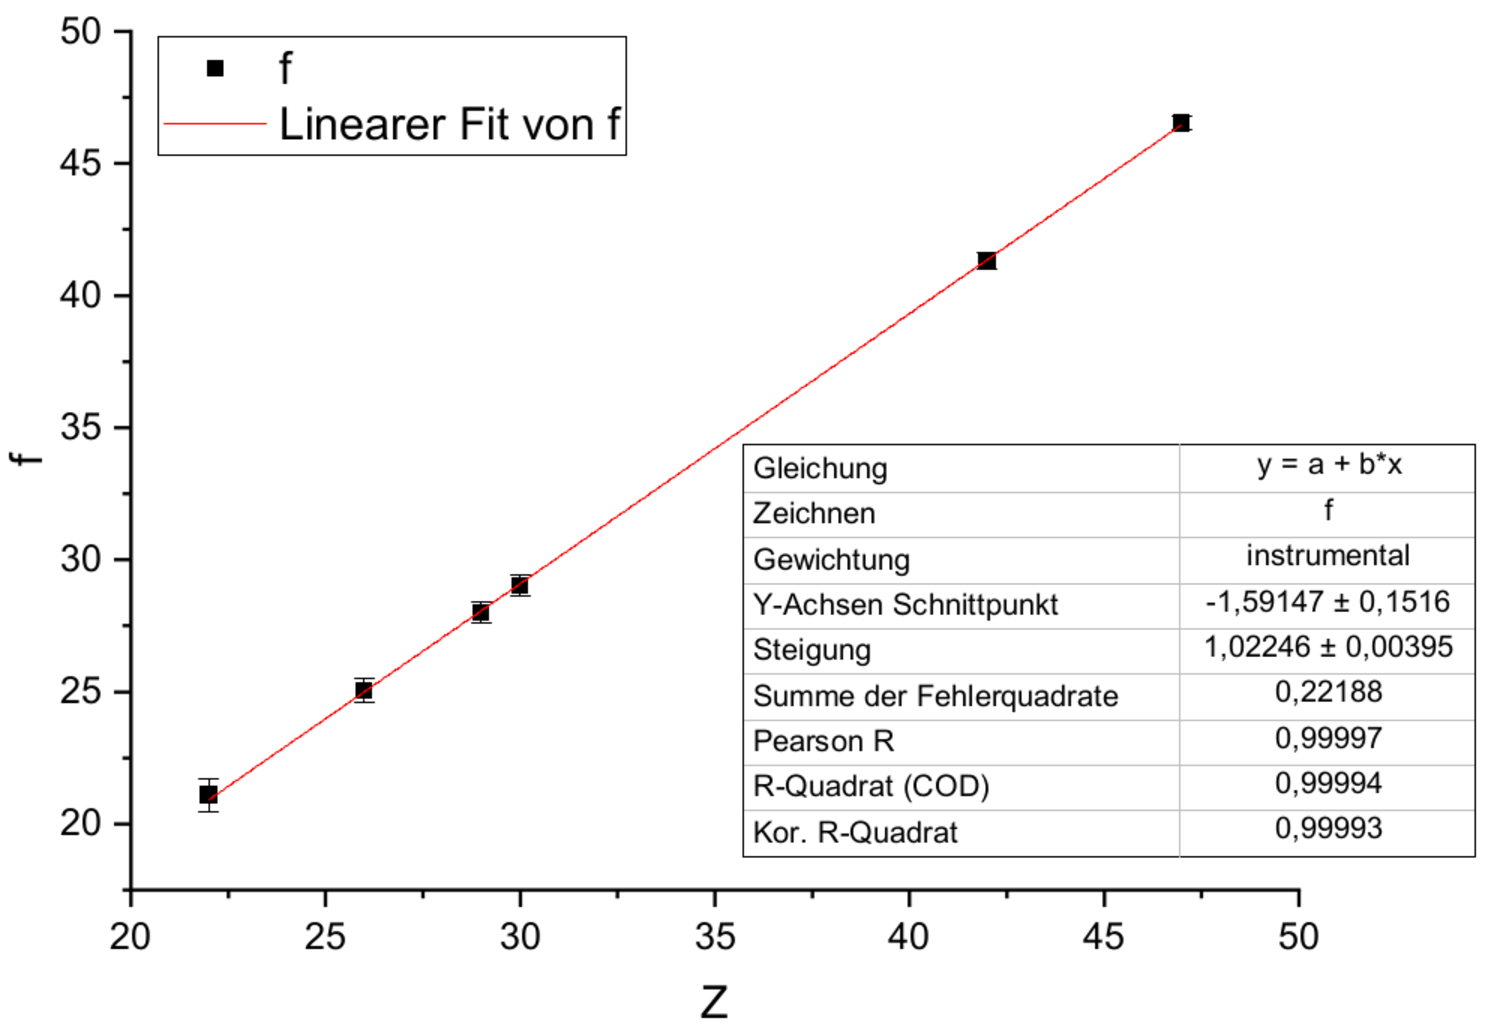
\includegraphics[width=0.9\textwidth]{Ka}
		\centering
		\caption{Die $\text{K}_\alpha$ Übergangsenergien wurden gemäß \cref{eq_f} umgeformt und gegen die Kernladungszahl $Z$ aufgetragen. Dabei beträgt $n_1=1$ und $n_2=2$.}
		\label{fig_Ka}
		\centering
	\end{figure}
	
	\begin{figure}[H]
		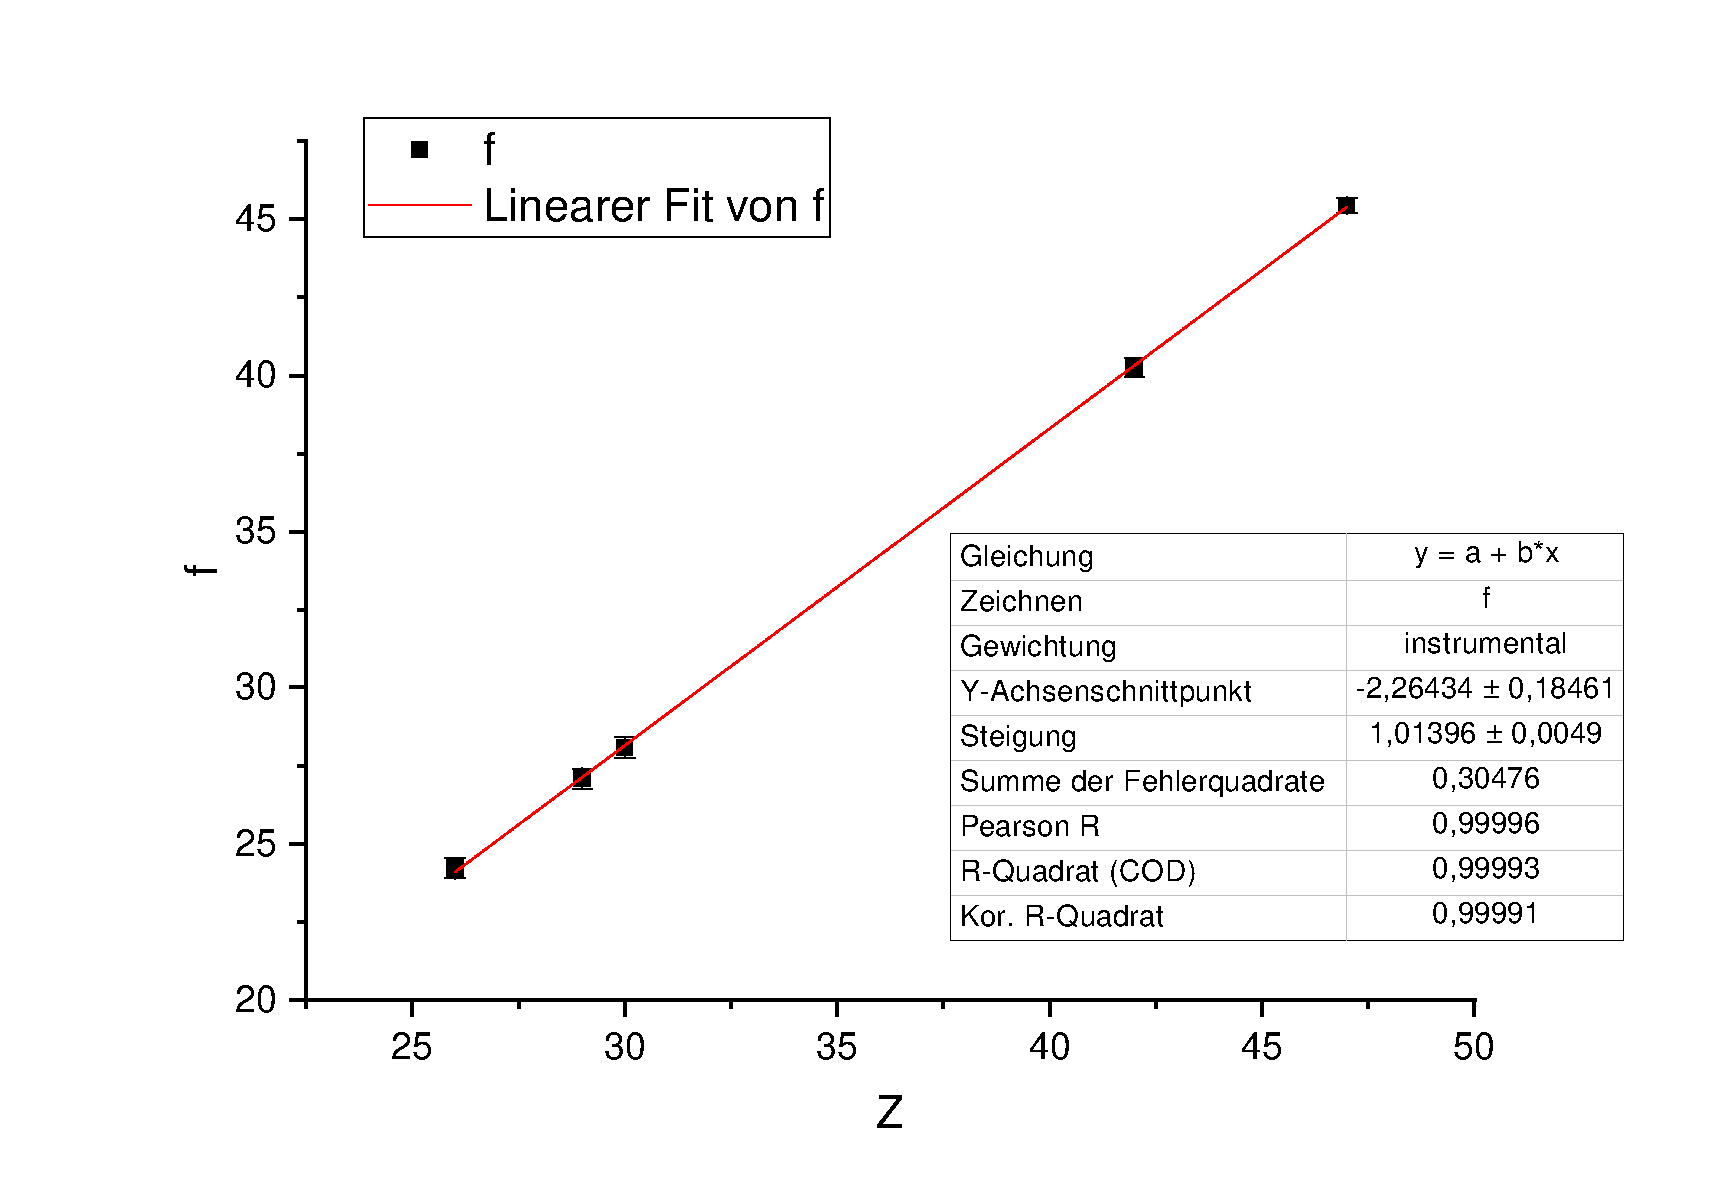
\includegraphics[width=0.9\textwidth]{Kb}
		\centering
		\caption{Die $\text{K}_\beta$ Übergangsenergien wurden gemäß \cref{eq_f} umgeformt und gegen die Kernladungszahl $Z$ aufgetragen. Dabei beträgt $n_1=1$ und $n_2=3$.}
			\label{fig_Kb}
			\centering
	\end{figure}
	
	Die y-Achsenabschnitte entsprechen $a=-\sigma_{n21}$ und sind die über alle Messpunkte gemittelte Abschirmkonstante.
	Anstelle derer bietet es sich an $\sigma_{n21}$ einzeln zu berechnen, da sie sich mit der Kernladungszahl $Z$ ändert.
	Die Ergebnisse von $\sigma_{n21}=Z-f$ sind in \cref{tb_abschirm} aufgeführt.
	
	\begin{table}[H]
		\centering
		\begin{tabular}{ c | c | c}
			Element & $\sigma_{n21}$ ($\text{K}_\alpha$) &  $\sigma_{n21}$ ($\text{K}_\beta$)\\ \hline \hline
			Ti & \SI{0,90249+-0,62796}{} & - \\
			Fe & \SI{0,96914+-0,46097}{} & \SI{1,7825+-0,32563}{} \\
			Cu & \SI{0,99347+-0,40884}{} & \SI{1,90376+-0,31974}{} \\
			Zn & \SI{0.98337+-0.39403}{} & \SI{1.91847+-0.3262}{} \\
			Mo & \SI{0,71061+-0,31317}{} & \SI{1,75324+-0,29969}{} \\
			Ag & \SI{0,48772+-0,26081}{} & \SI{1,56051+-0,24059}{} \\		
		\end{tabular}
	\caption{Die nach dem Moseleyschen Gesetz bestimmten Abschirmkonstanten der gemessenen $\text{K}_\alpha$ bzw. $\text{K}_\beta$ Übergänge.}
	\label{tb_abschirm} 
	\end{table}	

	\subsubsection{Bestimmung der Zusammensetzung}
	\begin{table}[H]
		\centering
		\resizebox{\textwidth}{!}{
		\begin{tabular}{ c | c || c | c | c }
			Probe (Angabe)&Energie $E$ in \SI{}{keV} & vermt. Element & char. Übergang &  Energie $E$ in \SI{}{keV} \\ \hline \hline					
			
			4 (20 Cent)
			& \SI{7.98262+-0.224069}{} &Cu &$\text{K}_\alpha$&   \SI{8. 0278416(26) }{} \\
			& \SI{8.7734+-0.247708}{} &Cu &$\text{K}_\beta$&  \SI{8 .905413(38) }{} \\ 
			\hline
			
			5 (Zn-Edelstahl)
			& \SI{6.41683+-0.35613}{} &Zn&?&\SI{ 6.38034+-0.278836    }{}* \\ 
			& \SI{8.5778+-0.252635}{} &Zn &$\text{K}_\alpha$&  \SI{8.615823(73)}{} \\
			& \SI{9.53652+-0.22887}{} &Zn &$\text{K}_\beta$ &  \SI{9.57203(22)}{}  \\
			\hline
			
			6 (Edelstahl)
			& \SI{3.39677+-0.379146}{} &Fe& ?  &  \SI{3.44288+-0.335591    }{}* \\ 
			& \SI{6.36975+-0.246009}{} & Fe & $\text{K}_\alpha$ &  \SI{6.3910264(99)}{}  \\
			& \SI{7.07128+-0.203035}{} &Fe& $\text{K}_\beta$&  \SI{7.058175(99)}{} \\
			\hline
			
			9 
			& \SI{6.36714+-0.297413}{} &Zn&?$&\SI{ 6.38034+-0.278836    }{}* \\
			& \SI{8.57041+-0.24602}{} &Zn &$\text{K}_\alpha$&  \SI{8.615823(73)}{}  \\ 
			& \SI{9.52768+-0.218296}{} &Zn &$\text{K}_\beta$ &  \SI{9.57203(22)}{} \\
			\hline
			
			10 
			& \SI{7.4251+-0.243006}{} &Ni & K$_\alpha$&  \SI{ 7. 4610343(45)     	}{} \\
			& \SI{8.23717+-0.212733}{} &Ni &K$_\beta$&  \SI{ 8. 264775(17)    }{} \\ 
			\hline
			
			11 
			& \SI{5.92928+-0.455814}{} &Ho & L$_\alpha$&  \SI{ 5. 939963(71)}{} \\ 
			& \SI{7.79736+-0.404885}{} &Ho & L$_\beta$& \SI{7 .76352(49) }{} \\
			& \SI{9.00316+-0.164444}{} &Ho & L$_\beta$& \SI{9 .0511(20) }{} \\
			\hline
			
			12 
			& \SI{9.11464+-0.376278}{} &Pb &L$_\alpha$&  \SI{9 .18456(70)    }{} \\ 
			& \SI{10.5011+-0.261044}{} &Pb &L$_\alpha$&  \SI{10. 55160(27)     }{} \\
			& \SI{12.562+-0.289138}{} &Pb &L$_\beta$&  \SI{ 12 .6012(13)     }{} \\
			& \SI{14.7821+-0.364269}{} &Pb &L$_\beta$&  \SI{  14 .7915(52)    }{} \\
			\hline
			
			13 
			& \SI{4.7454+-0.480512}{} & I & $\text{L}_\beta$ & \SI{4,66608(23)}{} \\
			& \SI{8.00052+-0.25263}{} & Cu & $\text{K}_\alpha$ &  \SI{8,0278416(26)}{}\\
			& \SI{8.88531+-0.246938}{} & Cu &  $\text{K}_\beta$ & \SI{8,905413(38)}{}\\
			& \SI{14.8774+-0.26906}{} & Y & $\text{K}_\alpha$ & \SI{14,88294(26)}{} \\
			& \SI{16.7011+-0.297662}{} & Y & $\text{K}_\beta$ &  \SI{16,6447(12)}{} \\ 
			\hline
			
			14 
			& \SI{3.07729+-0.327119}{} &Ag &  $\text{L}_\alpha$ &  \SI{3,150974(36) }{} \\
			& \SI{7.7277+-0.526665}{} & Co & $\text{K}_\beta$ &  \SI{7,70598(21)}{} \\
			& \SI{11.8938+-0.476134}{} & Au & $\text{L}_\beta $ & \SI{11,8287(14) }{} \\
			& \SI{15.0918+-0.63684}{} & Pb & $\text{L}_\beta $ &  \SI{15,1014(54)}{} \\
			& \SI{18.1496+-0.886139}{} & Zr & $\text{L}_\gamma $ &  \SI{17,9943(19)}{} \\
			& \SI{22.0709+-0.283243}{} &Ag & $\text{K}_\alpha$ &  \SI{21,99030(10)}{} \\
			& \SI{24.9643+-0.334121}{} &Ag & $\text{K}_\beta$ &  \SI{24,94242(30)}{} \\ 
			\hline
			
			15 
			& \SI{7.99436+-0.251832}{} & Cu & $\text{K}_\alpha$ &  \SI{8,0278416(26)}{} \\
			& \SI{8.88485+-0.218074}{} &  Cu &  $\text{K}_\beta$ & \SI{8,905413(38)}{} \\ 
			\hline
			
			16 (1-Cent)
			& \SI{7.98818+-0.234997}{} & Cu & $\text{K}_\alpha$ &  \SI{8,0278416(26)}{} \\
			& \SI{8.8637+-0.214616}{} & Cu &  $\text{K}_\beta$ & \SI{8,905413(38)}{} \\ 
			\hline
			
			17 
			& \SI{7.98377+-0.225856}{} & Cu & $\text{K}_\alpha$ & \SI{8,0278416(26)}{} \\
			& \SI{8.85058+-0.213236}{} & Cu & $\text{K}_\beta$ & \SI{8,905413(38)}{} \\ 
			\hline
			
			18 
			& \SI{7.41993+-0.228314}{} & Ni & $\text{K}_\alpha$ & \SI{7,4610343(45)}{} \\
			& \SI{8.21747+-0.205213}{} & Ni & $\text{K}_\beta$ &   \SI{8,264775(17)}{} \\ 
			\hline
			
			19 
			& \SI{5.40493+-0.248856}{} & Cr & $\text{K}_\alpha$ & \SI{5,4055384(71)}{} \\
			& \SI{6.33056+-0.227739}{} & Fe & $\text{K}_\alpha$ & \SI{ 6,3910264(99)}{} \\
			& \SI{7.05903+-0.435629}{} & Fe &  $\text{K}_\beta $ & \SI{7,058175(16)}{} \\ 
			\hline
			
			20 (Kronkorken) 
			& \SI{4.52319+-0.305646}{} & Sn & $\text{L}_\beta $ &  \SI{4,37683(46)}{} \\ %Ti wäre näher dran
			& \SI{6.35883+-0.22392}{} & Fe & $\text{K}_\alpha $ &  \SI{6,3910264(99)}{} \\
			& \SI{7.03423+-0.206604}{} & Fe & $\text{K}_\beta $ &  \SI{7,058175(16)}{} \\ 
			\hline
		\end{tabular}
		}
		\caption{Gemessene Röntgenfluoreszenzmaxima. Die charakteristischen Übergangsenergien sind die experimentellen Werte aus \cite{XRAYDB}, außer die mit einem * gekennzeichneten. Diese sind Messwerte aus \cref{tb_peaks_known}.} %TODO auch hier die E_index wie oben?
		\label{tb_peaks_unknown}
		
	\end{table}
	
	\subsection{Diskussion}
	%TODO Bezug/Nutzen oder sonst was
	%TODO auch hier die Hypothese wiederholen
	%TODO keine Messwerte hier, nach manchen Menschen, zumindest "direkt" erstellte Diagramme net hier, auch wenn Lesbarkeit-bla
	
	
	\section{Schlussfolgerung}
	%TODO Rückgriff auf Hypothese und drittes Nennen dieser
	
	%TODO Kritik: Häufig nicht eindeutig und nur mit Annahmen zuordnebar
	
	%TODO Quellen zitieren, Websiten mit Zugriffsdatum
	%TODO Verweise auf das Laborbuch (sind erlaubt)
	%TODO Tabelle + Bilder mit Beschriftung
	\printbibliography
\end{document}
